\documentclass[submit]{harvardml}

% FDV: Make sure all front matter has correct years, dates, book sections, etc.
\course{CS181-S22}
\assignment{Assignment \#2}
\duedate{7:59pm EST, Feb 25th, 2022}

\usepackage[OT1]{fontenc}
\usepackage[colorlinks,citecolor=blue,urlcolor=blue]{hyperref}
\usepackage[pdftex]{graphicx}
\usepackage{subfig}
\usepackage{fullpage}
\usepackage{amsmath}
\usepackage{amssymb}
\usepackage{framed}
\usepackage{color}
\usepackage{soul}
\usepackage{todonotes}
\usepackage{listings}
\usepackage{common}
\usepackage{enumitem}
\usepackage{bm}
\usepackage{bbm}
\newcommand{\B}{\text{B}}
\newcommand{\Beta}{\text{Beta}}

\usepackage[mmddyyyy,hhmmss]{datetime}

\definecolor{verbgray}{gray}{0.9}

\lstnewenvironment{csv}{%
  \lstset{backgroundcolor=\color{verbgray},
  frame=single,
  framerule=0pt,
  basicstyle=\ttfamily,
  columns=fullflexible}}{}

\begin{document}

\begin{center}
{\Large Homework 2: Classification and Bias-Variance Trade-offs}\\
\end{center}

\subsection*{Introduction}

This homework is about classification and bias-variance trade-offs. In
lecture we have primarily focused on binary classifiers trained to
discriminate between two classes. In multiclass classification, we
discriminate between three or more classes.  Most of the material for Problem 1 and Problem 3, and all of the material for Problem 2 will be covered by the end of the Tuesday 2/8 lecture. The rest of the material will be covered by the end of the Thursday 2/10 lecture.  We encourage you to read
CS181 Textbook's Chapter 3 for more information on linear
classification, gradient descent, classification in the discriminative
setting (covers multiclass logistic regression and softmax), and
classification in the generative setting. Read Chapter 2.8 for more
information on the trade-offs between bias and variance.

As a general note, for classification problems we imagine that we have
the input matrix $\boldX \in \reals^{N \times D}$ (or perhaps they
have been mapped to some basis $\bm{\Phi}$, without loss of
generality) with outputs now ``one-hot encoded."  This means that if
there are~$K$ output classes, rather than representing the output
label $y$ as an integer~${1,2,\ldots,K}$, we represent $\boldy$ as a
``one-hot" vector of length~$K$. A ``one-hot" vector is defined as
having every component equal to 0 except for a single component which
has value equal to 1.  For example, if there are $K = 7$ classes and a
particular data point belongs to class 3, then the target vector for
this data point would be~$\boldy = [0,0,1,0,0,0,0]$.  We will define
$C_1$ to be the one-hot vector for the 1st class, $C_2$ for the 2nd
class, etc.  Thus, in the previous example $\boldy = C_3$. If there
are $K$ total classes, then the set of possible labels is $\{C_1
\ldots C_K \} = \{C_k\}_{k=1}^K$.  Throughout the assignment we will
assume that each label $\boldy \in \{C_k\}_{k=1}^K$ unless otherwise
specified. The most common exception is the case of binary classification
($K = 2$), in which case labels are the typical integers $y \in \{0, 1\}$.\\

In problems 1 and 3, you may use \texttt{numpy} or \texttt{scipy}, but
not \texttt{scipy.optimize} or \texttt{sklearn}. Example code given is
in Python 3.\\

Please type your solutions after the corresponding problems using this
\LaTeX\ template, and start each problem on a new page.\\

Please submit the \textbf{writeup PDF to the Gradescope assignment `HW2'}. Remember to assign pages for each question.  \textbf{You must include your plots in your writeup PDF. } The supplemental files will only be checked in special cases, e.g. honor code issues, etc. \\

Please submit your \textbf{\LaTeX\ file and code files to the Gradescope assignment `HW2 - Supplemental'}. 

%%%%%%%%%%%%%%%%%%%%%%%%%%%%%%%%%%%%%%%%%%%%%
% Problem 1
%%%%%%%%%%%%%%%%%%%%%%%%%%%%%%%%%%%%%%%%%%%%%

\begin{problem}[Exploring Bias and Variance, 10 pts]
  In this problem, we will explore the bias and variance of a
  few different model classes when it comes to logistic regression.

  Consider the true data generating process $y \sim \text{Bern}(f(x)), f(x) = 0.4 \times \sin(1.2x) + 0.5$, where $x \in [-3, 3]$, and $y \in \{0,1\}$.
  Recall that for a given $x$, bias and variance are defined in terms of expectations \textit{over randomly drawn datasets} $D$
  from this underlying data distribution:
  \begin{align*}
  \text{Bias}[\hat{f}(x)] &= \mathbb{E}_D[\hat{f}(x)] - f(x)\\
  \text{Variance}[\hat{f}(x)] &= \mathbb{E}_D[(\hat{f}(x) - \mathbb{E}_D[\hat{f}(x)])^2]
  \end{align*}
  Here, $\hat{f}(x)$ is our estimator (learned through logistic
  regression on a given dataset $D$).  We will directly explore the
  bias-variance trade-off by drawing multiple such datasets and
  fitting different logistic regression models to each.  Remember that
  we, the modelers, do not usually see the true data distribution.
  Knowledge of the true $f(x)$ is only exposed in this problem to (1)
  make possible the simulation of drawing multiple datasets, and (2)
  to serve as a pedagogical tool in allowing verification of the true
  bias.

\begin{enumerate}

\item Consider the three bases $\phi_1(x) = [1, x]$, $\phi_2(x) = [1,
  x, x^2]$, $\phi_3(x) = [1, x, x^2, x^3, x^4, x^5]$.  For each
  of these bases, generate 10 datasets of size $N = 30$ using the
  starter code provided, and fit a logistic regression model using
  sigmoid($w^T \phi(x)$) to each dataset by using gradient descent to
  minimize the negative log likelihood.  This means you will be
  running gradient descent 10 times for each basis, once for each
  dataset.  Note that the classes are represented with 0's and 1's.
  
  Use random starting values of $w$, $\eta=0.001$, take 10,000 update
  steps for each gradient descent run, and make sure to average the
  gradient over the data points (for each step). These parameters,
  while not perfect, will ensure your code runs in a reasonable amount
  of time. The emphasis of this problem is on capturing the
  bias-variance trade-off, so don't worry about attaining perfect
  precision in the gradient descent as long as this trade-off is
  captured in the final models.

   Note: Overflow RuntimeWarnings due to \verb|np.exp| should be safe to ignore, if any. Also, to reduce stress from randomness in students' solutions (due to randomized weight initialization differences), in line $109$ of the \verb|T2_P1.py| starter code, we call \verb|np.random.seed(1738)| to set a deterministic random seed. Please do not change this! In addition, please do not change the randomized weight initialization code in lines $42-46$.

\item Create three plots, one for each basis. Starter code is available which you may modify.
By default, each plot displays three types of functions:
(1) the true data-generating distribution $f(x)$ (the probability that $y=1$ for different $x$).
(2) all 10 of the prediction functions learned from each randomly drawn dataset, and
(3) the mean of the 10 prediction functions.
Moreover, each plot also displays 1 of the randomly generated datasets and highlights the corresponding prediction function learned by this dataset.

\item How are bias and variance reflected in the 3 types of curves on
  the graphs?  How do the fits of the individual and mean prediction
  functions change?  Keeping in mind that none of the model classes
  match the true generating process exactly, discuss the extent to
  which each of the bases approximates the true process.

  Note: In this problem, we are not interested in whether the model is
  more biased for certain inputs $x$ compared to other inputs $x'$.
  We are interested in the overall bias and variance of $\hat{f}(x)$
  across the different basis choices. In other words, we want to investigate how the bias between $\hat{f}(x)$ and the ground truth as well as the variance of $\hat{f}(x)$ will be different over different basis choices. 

\item If we were to increase the size of each dataset drawn from $N = 10$ to a larger number, how would the variance change? The bias?   Why might this be the case?

\end{enumerate}

\end{problem}

\newpage

\subsection*{Solution}
\noindent\textbf{Solution 1.1:}\\
See \verb|T2_P1.py| in Gradescope HW2 - Supplemental.\\

\noindent\textbf{Solution 1.2:}\\
\begin{center}
    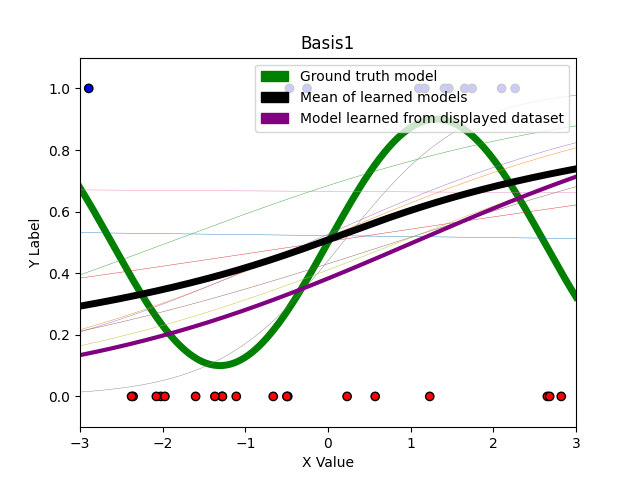
\includegraphics[scale=0.7]{Basis1.png}
\end{center}
\begin{center}
    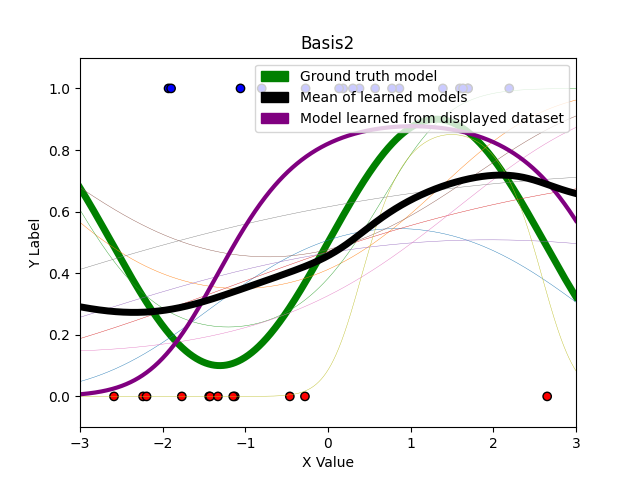
\includegraphics[scale=0.7]{Basis2.png}
\end{center}
\begin{center}
    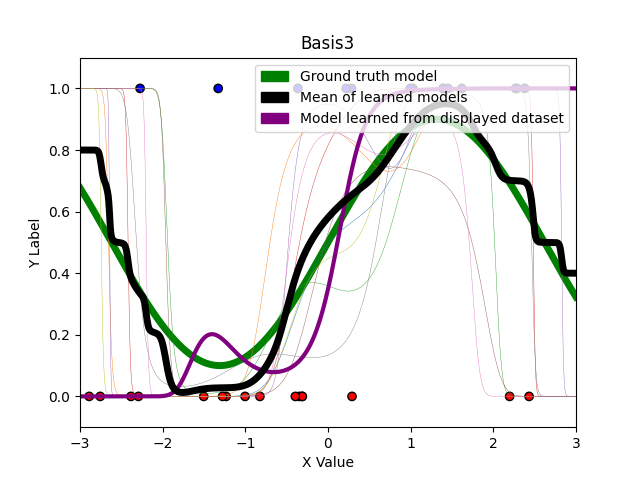
\includegraphics[scale=0.7]{Basis3.png}
\end{center}

\noindent\textbf{Solution 1.3:}\\
Bias is depicted by the difference between the black line (mean learned model) and green line (ground truth model), while variance is depicted by the variation of the purple line/faint lines in the background (individual learned models) from the black line. 

It is clear that that Basis1 is underfitting the data, as it produces a very simple mean learned model (the average of linear learned models); it has high bias (the mean learned model is hardly similar to the ground truth model) but low variance (the individual learned models are very similar to the mean learned model). By comparison, Basis3 is overfitting the data as it produces a more complicated mean learned model (the average of 5th order polynomials); it has a low bias (the mean learned model is more similar to the ground truth model) but high variance (the individual learned models have a large spread from the mean learned model, e.g. look at the difference between the purple and black lines to the left of the figure). Basis2's learned model (the average of 3rd order polynomials) has a bias and variance in between Basis1 and Basis3.

Overall, this is in line with the theory of more complicated models having low bias and high variance, whilst simpler models have high bias and low variance. Basis1 arguably fits the data least well because a linear model simply cannot predict the features of the sinusoidal ground truth model. Basis3 arguably approximates the true process best because it has low bias, but it is also arguably overfitting and suffers from high variance. Basis2 arguably best optimizes for the bias-variance tradeoff - it follows the ground truth model more closely (lower bias) than Basis1, and the individual learned models are closer to the mean learned model (lower variance) than Basis3.\

\noindent\textbf{Solution 1.4:}\\
Increasing the number of data points in the training data can decrease the variance. This will be more pronounced in the case of Basis3, which has a higher variance and will be more sensitive to the addition of additional training data (it will effectively overfit to the additional data, leading to the individual learned models being closer to the mean learned model). 

However, increasing the number of data points will not change the bias because the bias is caused by the features of the model rather than the amount of data we have to fit to. For example, Basis1 produces linear models; a line that is a better weighted average of more training data will not result in a curve that begins to look sinusoidal - it's still a line!

%%%%%%%%%%%%%%%%%%%%%%%%%%%%%%%%%%%%%%%%%%%%%
% Problem 2
%%%%%%%%%%%%%%%%%%%%%%%%%%%%%%%%%%%%%%%%%%%%%
\begin{problem}[Maximum likelihood in classification, 15pts]

  Consider now a generative $K$-class model.  We adopt class prior
  $p(\boldy = C_k; \bpi) = \pi_k$ for all $k \in \{1, \ldots, K\}$
(where $\pi_k$ is a parameter of the prior).
Let  $p(\boldx|\boldy=C_k)$ denote
the class-conditional density of features $\boldx$ (in this
case for class $C_k$). Consider the data set $D = \{(\boldx_i,
\boldy_i)\}_{i=1}^n$ where as above $\boldy_i \in \{C_k\}_{k=1}^K$ is
encoded as a one-hot target vector and the data are independent.

\begin{enumerate}
  \item Write out the log-likelihood of the data set, $\ln p(D ; \bpi)$.

  \item Since the prior forms a distribution, it has the constraint that
    $\sum_k\pi_k - 1 = 0$.  Using the hint on
Lagrange multipliers below, give the
    expression for the maximum-likelihood estimator for the prior
    class-membership probabilities, i.e.
    $\hat \pi_k.$
    Make sure to write out the intermediary equation you need
    to solve to obtain this estimator. Briefly state why your final answer is intuitive.
\end{enumerate}

    For the remaining questions, let the
    class-conditional probabilities be Gaussian distributions with
the same covariance matrix
    $$p(\boldx | \boldy = C_k) = \mathcal{N}(\boldx |  \bmu_k, \bSigma), \text{\ for\ }k \in \{1,\ldots, K\}$$
    and different means $\bmu_k$ for each class.

    \begin{enumerate}
  \item[3.] Derive the gradient of the log-likelihood with respect to vector $\bmu_k$.
    Write the expression in matrix form as a function of the variables defined
    throughout this exercise. Simplify as much as possible for full credit.
  \item[4.] Derive the maximum-likelihood estimator $\hat{\mu}_k$ for vector $\bmu_k$. Briefly state why your final answer is intuitive.
  \item[5.] Derive the gradient for the log-likelihood with respect to the
    covariance matrix $\bSigma$ (i.e., looking
to find an MLE for the covariance).
Since you are differentiating with respect to a
    \emph{matrix}, the resulting expression should be a matrix!
%
  \item[6.] Derive the maximum likelihood estimator $\hat{\Sigma}$ of the covariance matrix.
\end{enumerate}

\paragraph{Hint: Lagrange Multipliers.} Lagrange Multipliers are a method for
optimizing a function $f$ with respect to an
equality constraint, i.e.
\[\min_{\boldx} f(\boldx)\ \text{s.t.}\ g(\boldx) = 0.\]

This can be turned into an unconstrained problem by introducing a
Lagrange multiplier $\lambda$ and constructing the Lagrangian function,
\[L(\boldx, \lambda) =  f(\boldx) + \lambda g(\boldx).\]

It can be shown that it is a necessary condition that the optimum
is a critical point of this new function. We can find this point by solving two equations:

\[\frac{\partial L(\boldx, \lambda)}{\partial  \boldx} = 0  \ \ \text{and}\  \  \frac{\partial L(\boldx, \lambda)}{\partial \lambda} = 0 \]


\paragraph{Cookbook formulas.} Here are some formulas you might want to consider
using to compute difficult gradients. You can use them  in the homework
without proof. If you are looking to hone your matrix calculus skills, try to
find different ways to prove these formulas yourself (will not be part of the
evaluation of this homework). In general, you can use any formula from the matrix cookbook,
as long as you cite it. We opt for the following common notation:
$\boldX^{-\top} := (\boldX^{\top})^{-1}$
\begin{align*}
  & \frac{\partial \bolda^\top \boldX^{-1} \boldb}{\partial \boldX} = - \boldX^{-\top} \bolda \boldb^\top \boldX^{-\top} \\
  & \frac{\partial \ln | \det (\boldX) |}{\partial \boldX} = \boldX^{-\top}
 \end{align*}
 \end{problem}


\subsection*{Solution}

\noindent\textbf{Solution 2.1:}\\
The likelihood of the data set is given by:
\begin{align*}
    p(D ; \bpi) &= p(\{(\boldx_i, \boldy_i)\}_{i=1}^n; \bpi)\\
    &= \prod_{i=1}^{n} p(\{(\boldx_i, \boldy_i)\}_{i=1}; \bpi)
\end{align*}

In order to calculate this probability, consider the probability of seeing one data point given the parameters:
\begin{align*}
    p(\{(\boldx_i, \boldy_i)\}; \bpi) &= \prod_{k=1}^{K} p(\{\boldx_i; \boldy_i = C_k, \bpi) p(\boldy_i = C_k; \bpi)\\
    &= \prod_{k=1}^{K} p(\{\boldx_i; \boldy_i = C_k, \bpi)  \bpi_k
\end{align*}

Therefore, the likelihood of the data set can be re-written as:
\begin{align*}
    p(D ; \bpi) &= \prod_{i=1}^{n} \prod_{k=1}^{K} p(\{\boldx_i; \boldy_i = C_k, \bpi)  \bpi_k
\end{align*}

Taking the log of the likelihood, we can convert logarithms of products to sums of logarithms multiplied by the indicator $\mathbbm{1}_{\boldy_i = C_k}$, such that we only sum the logarithms of probabilities for data that are in the correct class. Thus, we get the log-likelihood of the data set:
\begin{align*}
    \ln p(D ; \bpi) &= \sum_{i=1}^{n} \sum_{k=1}^{K} (\ln[p(\{\boldx_i; \boldy_i = C_k, \bpi)] + \ln[\bpi_k]) \mathbbm{1}_{\boldy_i = C_k}
\end{align*}

\noindent\textbf{Solution 2.2:}\\
To find the maximum-likelihood estimator for the prior probabilities, we solve the following constrained optimization problem:
\begin{align*}
    \max_{\bpi} p(D ; \bpi)\  \text{s.t.}\ \sum_{k=1}^{K}\pi_k - 1 = 0
\end{align*}

Turning this into an unconstrained maximization problem using a Lagrangian yields:
\begin{align*}
    L(\bpi_k, \lambda) = \sum_{i=1}^{n} \sum_{k=1}^{K} (\ln[p(\{\boldx_i; \boldy_i = C_k, \bpi)] + \ln[\bpi_k]) \mathbbm{1}_{\boldy_i = C_k} + \lambda ( \sum_{k=1}^{K}\pi_k - 1)
\end{align*}

Now, take the derivative with respect to $\lambda$ and take K derivatives with respect to $\bpi_1, ..., \bpi_K$:
\begin{align*}
    \frac{\delta L}{\delta \lambda} &= \sum_{k=1}^{K}\pi_k - 1\\
    \frac{\delta L}{\delta \bpi_k} &= \sum_{i=1}^{n} \frac{1}{\bpi_k} \mathbbm{1}_{\boldy_i = C_k} + \lambda
\end{align*}

The Lagrangian is maximized when these derivatives equal 0:
\begin{align}
    \sum_{k=1}^{K}\pi_k &= 1\\
    \sum_{i=1}^{n} \frac{1}{\bpi_k} \mathbbm{1}_{\boldy_i = C_k} &= - \lambda
\end{align}

Rearranging equation (2):
\begin{align*}
    \bpi_k &= - \frac{1}{\lambda}\sum_{i=1}^{n} \mathbbm{1}_{\boldy_i = C_k}\\
    &= - \frac{1}{\lambda} N_k
\end{align*}
where $N_k$ is defined as the number of data points $(\boldx_i,
\boldy_i)$ in class $k$.\\

Substituting this into equation (1):
\begin{align*}
    \sum_{k=1}^{K} \frac{1}{\lambda} N_k &= 1\\
    - \sum_{k=1}^{K} N_k &= \lambda\\
    \lambda = -N
\end{align*}
where $N$ is defined as the number of data points $(\boldx_i,
\boldy_i)$ in the data set.\\

Putting this all together, we get maximum-likelihood estimator for the prior class-membership probabilities, $\hat \pi_k$:
\begin{align*}
    \hat \pi_k = \frac{N_k}{N}
\end{align*}

This is intuitive because the probability of being in a given class $C_k$ equals the number of data points in that class $N_k$ divided by the total number of data points $N$ (i.e. the fraction of data points that are assigned to class $C_k$).\\

\noindent\textbf{Solution 2.3:}\\
Given $p(\boldx | \boldy = C_k) = \mathcal{N}(\boldx |  \bmu_k, \bSigma)$, the log-likelihood can be rewritten as:
\begin{align*}
    \ln p(D ; \bpi) &= \sum_{i=1}^{n} \sum_{k=1}^{K} (\ln[\mathcal{N}(\boldx |  \bmu_k, \bSigma)] + \ln[\bpi_k]) \mathbbm{1}_{\boldy_i = C_k}\\
\end{align*}

The Gaussian distribution can be re-written in terms of its PDF, abstracting all terms not containing $\bmu_k$ into a constant $c$:
\begin{align*}
    \ln p(D ; \bpi) &= \sum_{i=1}^{n} \sum_{k=1}^{K} (-\frac{1}{2} (\boldx_i - \bmu_k)^{\top} \bSigma^{-1}(\boldx_i - \bmu_k) + c) + \ln[\bpi_k]) \mathbbm{1}_{\boldy_i = C_k}
\end{align*}

Using the Matrix Cookbook formulae yields the gradient of the log-likelihood with respect to $\bmu_k$ for a given $k$:
\begin{align*}
    \nabla_{\bmu_k} \ln p(D ; \bpi) &= \sum_{i=1}^{n} \bSigma^{-1} (\boldx_i - \bmu_k) \mathbbm{1}_{\boldy_i = C_k}\\
    &= \bSigma^{-1}  (\sum_{i=1}^{n} [\boldx_i \mathbbm{1}_{\boldy_i = C_k}] - N_k \bmu_k)
\end{align*}

\noindent\textbf{Solution 2.4:}\\
The maximum-likelihood estimator $\hat \bmu_k$ for $\bmu_k$ is found by setting the gradient equal to 0:
\begin{align*}
    \bSigma^{-1}  (\sum_{i=1}^{n} \boldx_i \mathbbm{1}_{\boldy_i = C_k} - N_k \bmu_k) = 0\\
    \hat \bmu_k = \frac{1}{N_k} \sum_{i=1}^{n} \boldx_i \mathbbm{1}_{\boldy_i = C_k}\\
\end{align*}

This is intuitive as $\hat \bmu_k$ is simply the average of all the data points $\boldx_i$ assigned to class $C_k$.\\

\noindent\textbf{Solution 2.5:}\\
Recall the log-likelihood function with Gaussian class-conditional probabilities:
\begin{align*}
    \ln p(D ; \bpi) &= \sum_{i=1}^{n} \sum_{k=1}^{K} (\ln[\mathcal{N}(\boldx |  \bmu_k, \bSigma)] + \ln[\bpi_k]) \mathbbm{1}_{\boldy_i = C_k}\\
\end{align*}

The Gaussian distribution can be re-written in terms of its PDF, abstracting all terms not containing $\bSigma$ into a constant $c$:
\begin{align*}
    \ln p(D ; \bpi) &= \sum_{i=1}^{n} \sum_{k=1}^{K} (-\frac{1}{2} (\boldx_i - \bmu_k)^{\top} \bSigma^{-1}(\boldx_i - \bmu_k) - \frac{1}{2} \ln[\det(\bSigma)] + c) + \ln[\bpi_k]) \mathbbm{1}_{\boldy_i = C_k}
\end{align*}

Using the Matrix Cookbook formulae yields the gradient of the log-likelihood with respect to $\bSigma$:
\begin{align*}
    \nabla_{\bSigma} \ln p(D ; \bpi) &= \sum_{i=1}^{n} \sum_{k=1}^{K} (- \frac{1}{2} \bSigma^{-\top} (\boldx_i - \bmu_k)(\boldx_i - \bmu_k)^{\top}\bSigma^{-\top} + \frac{1}{2} \bSigma^{-\top}) \mathbbm{1}_{\boldy_i = C_k}\\
    &= - \frac{1}{2} \bSigma^{-\top} \sum_{i=1}^{n} \sum_{k=1}^{K} ((\boldx_i - \bmu_k)(\boldx_i - \bmu_k)^{\top}\bSigma^{-\top} - \boldI) \mathbbm{1}_{\boldy_i = C_k}\\
\end{align*}

\noindent\textbf{Solution 2.6:}\\
The maximum-likelihood estimator $\hat \bSigma$ for $\bSigma$ is found by setting the gradient equal to 0:
\begin{align*}
    - \frac{1}{2} \bSigma^{-\top} \sum_{i=1}^{n} \sum_{k=1}^{K} ((\boldx_i - \bmu_k)(\boldx_i - \bmu_k)^{\top}\bSigma^{-\top} - \boldI) \mathbbm{1}_{\boldy_i = C_k} = 0
\end{align*}

Multiplying both sides by $\bSigma^{\top}$ from the left and right (with the effect of
retaining $\bSigma^{\top}$ in only the second term, since $\bSigma^{\top} \bSigma^{-\top} = \bSigma^{-\top} \bSigma^{\top} = \boldI$), and multiplying by $-2$, we have:
\begin{align*}
    \sum_{i=1}^{n} \sum_{k=1}^{K} ((\boldx_i - \bmu_k)(\boldx_i - \bmu_k)^{\top} - \bSigma^{\top}) \mathbbm{1}_{\boldy_i = C_k} &= 0\\
    \sum_{i=1}^{n} \sum_{k=1}^{K} (\boldx_i - \bmu_k)(\boldx_i - \bmu_k)^{\top} \mathbbm{1}_{\boldy_i = C_k} &= N \bSigma^{\top}
\end{align*}

Rearranging to solve for $\hat \bSigma$, the maximum likelihood estimator for $\bSigma$, and recognizing that covariance matrices are symmetric, and so
$\bSigma^{\top} = \bSigma$, we have:
\begin{align*}
    \hat \bSigma = \frac{1}{N} \sum_{i=1}^{n} \sum_{k=1}^{K} (\boldx_i - \bmu_k)(\boldx_i - \bmu_k)^{\top} \mathbbm{1}_{\boldy_i = C_k}
\end{align*}

This is intuitive as the maximum likelihood solution for the shared covariance matrix is the weighted average of the individual covariance matrices for each class. Note that in the sum, we only include terms in the individual covariance matrices when the indicator $\mathbbm{1}_{\boldy_i = C_k} = 1$.

%%%%%%%%%%%%%%%%%%%%%%%%%%%%%%%%%%%%%%%%%%%%%
% Problem 3
%%%%%%%%%%%%%%%%%%%%%%%%%%%%%%%%%%%%%%%%%%%%%

\begin{problem}[Classifying Stars, 15pts]

You're tasked with classifying three different kinds of stars using their magnitudes and temperatures. See star.png for a plot of
the data, adapted from
\url{http://astrosci.scimuze.com/stellar_data.htm} and available as
\verb|data/hr.csv|, which you will find in the Github repository. \\

The CSV file has three columns: type, magnitude, and temperature. The
first few lines look like this:
\begin{csv}
Type,Magnitude,Temperature
Dwarf,-5.8,-0.35
Dwarf,-4.1,-0.31
...
\end{csv}

In this problem, you will code up 4 different classifiers for this task:
\begin{enumerate}[label=\alph*)]

\item \textbf{A three-class generalization of logistic regression},
  also known as softmax regression, in which you implement gradient
  descent on the negative log-likelihood. In Question 2 you will
  explore the effect of using different values for the learning rate
  $\eta$ (\texttt{self.eta}) and regularization strength $\lambda$
  (\texttt{self.lam}).  Make sure to include a bias term and to use L2
  regularization. See CS181 Textbook's Chapter 3.6 for details on  multi-class logistic regression and softmax. For your implementation, use the loss and gradient expressions provided there.

\item \textbf{A generative classifier with Gaussian class-conditional
  densities with a \textit{shared covariance} matrix} across all classes. 
  Feel free to re-use your Problem 2 results.
\item \textbf{Another generative classifier with Gaussian class-conditional densities , but now 
with a \textit{separate covariance} matrix} learned for each class. (Note: 
The staff implementation can switch between the two Gaussian generative classifiers with just a
few lines of code.)

\item \textbf{A kNN classifier} in which you classify based on the $k=1,3,5$ nearest neighbors and the following distance function: $$dist(star_1, star_2) = ((mag_1 - mag_2)/3)^2 + (temp_1 - temp_2)^2$$
where nearest neighbors are those with the smallest distances from a given point.

  Note 1: When there are more than two labels, no label may have the
  majority of neighbors.  Use the label that has the most votes among
  the neighbors as the choice of label. 

  Note 2: The grid of points for which you are making predictions
  should be interpreted as our test space.  Thus, it is not necessary
  to make a test point that happens to be on top of a training point
  ignore itself when selecting neighbors.

\end{enumerate}

After implementing the above classifiers, complete the following exercises:

\begin{enumerate}
    \item Plot the decision boundaries generated by each classifier for the dataset. Include them in your PDF. 
    Identify the similarities and differences among the classifiers. What explains the differences?

    \item For logistic regression only, make a plot with ``Number of
      Iterations" on the x-axis and ``Negative Log-Likelihood Loss" on
      the y-axis for several configurations of the hyperparameters
      $\eta$ and $\lambda$.  Specifically, try the values $0.05$,
      $0.01$, and $0.001$ for each hyperparameter.  Limit the number
      of gradient descent iterations to 200,000.  What are your final
      choices of learning rate ($\eta$) and regularization strength
      ($\lambda$), and why are they reasonable? How does altering
      these hyperparameters affect the ability to converge, the rate
      of convergence, and the final loss (a qualitative description is
      sufficient)? You only need to submit one plot for your final
      choices of hyperparameters.

      Note: The \emph{likelihood} of the model is the probability of
      data given the model---it should not include the regularization
      term.  The \emph{objective} is the combination of the likelihood
      and the regularizer.
      
    \item For both Gaussian generative models, report the negative log-likelihood loss. Which model has a lower loss, and why?
      For the separate covariance model, be sure to use
      the covariance matrix that matches the true class of each data
      point.
    
    \item Consider a star with Magnitude 6 and Temperature 2.
      To what class does each classifier assign this star? Do the
      classifiers give any indication as to whether or not you should
  trust them?
\end{enumerate}
\end{problem}

\newpage

\begin{framed}
\noindent\textbf{Problem 3} (cont.)\\


\textbf{Implementation notes:} Run the controller file, \texttt{T2\_P3.py},
to test your code. Write the actual implementations in the \texttt{GaussianGenerativeModel},
\texttt{LogisticRegression}, and \texttt{KNNModel} classes, which are defined in the three
\texttt{T2\_P3\_ModelName.py} files. These classes follow the same interface pattern
as sklearn. Their code
currently outputs nonsense predictions just to show the
high-level interface, so you should replace their \texttt{predict()} implementations.
You'll also need to modify the hyperparameter
values in \texttt{T2\_P3.py} for logistic regression.
\end{framed}

\newpage

\subsection*{Solution}
\noindent\textbf{Solution 3.1:}\\
(a) Three-class generalization of logistic regression
\begin{center}
    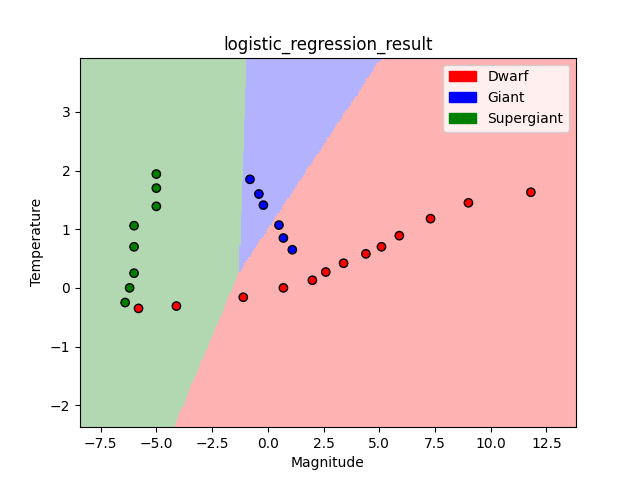
\includegraphics[scale=0.7]{logistic_regression_result.png}
\end{center}

(b) Generative classifier with Gaussian class-conditional densities with a \textit{shared} covariance matrix across all classes
\begin{center}
    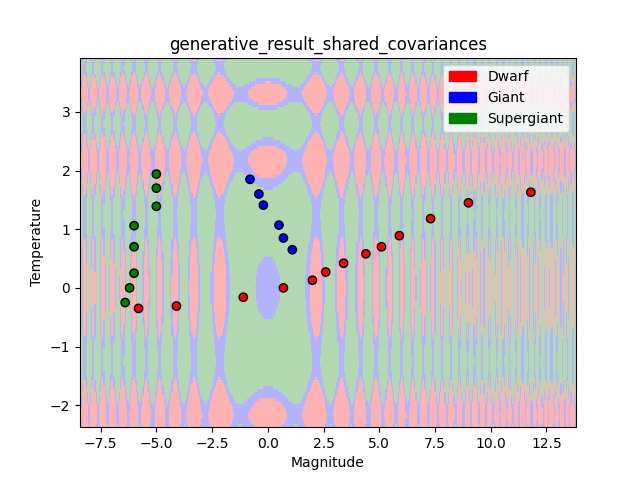
\includegraphics[scale=0.7]{generative_result_shared_covariances.png}
\end{center}

(c) Generative classifier with Gaussian class-conditional densities with a \textit{separate} covariance matrix for each class
\begin{center}
    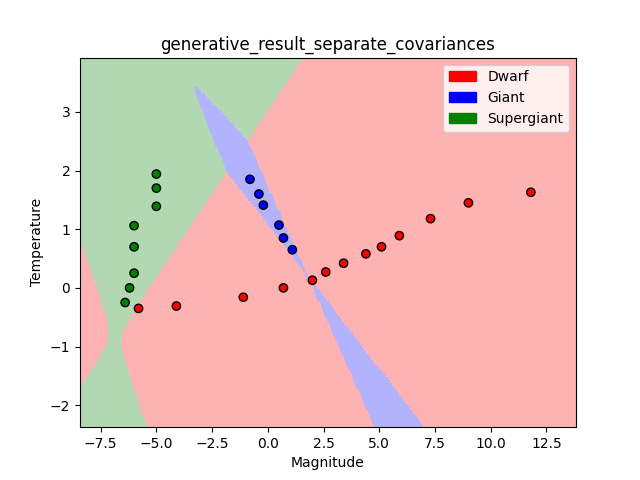
\includegraphics[scale=0.7]{generative_result_separate_covariances.png}
\end{center}

(d) kNN classifier based on $k = 1, 3, 5$ nearest neighbors
\begin{center}
    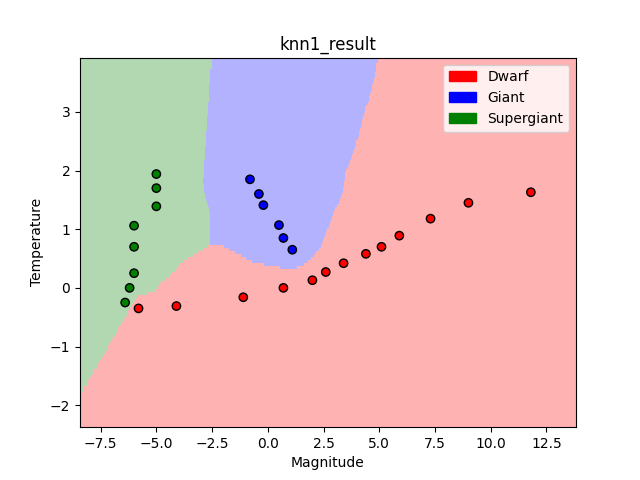
\includegraphics[scale=0.7]{HW2/knn1_result.png}
\end{center}
\begin{center}
    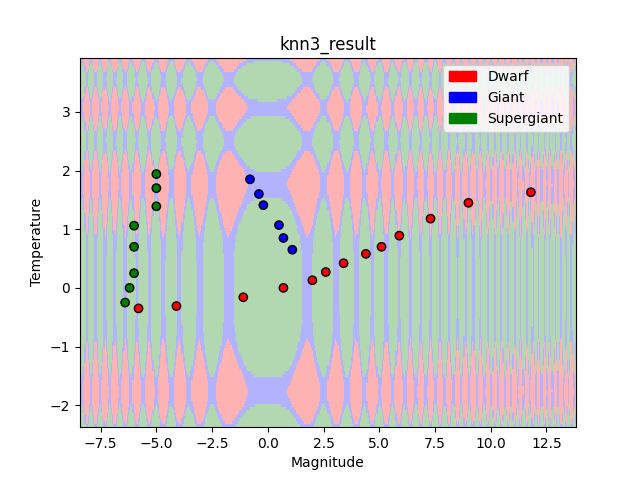
\includegraphics[scale=0.7]{HW2/knn3_result.png}
\end{center}
\begin{center}
    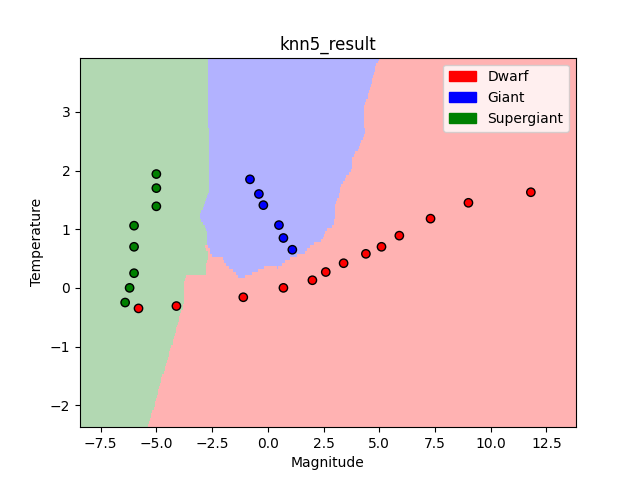
\includegraphics[scale=0.7]{HW2/knn5_result.png}
\end{center}

Logistic regression produces linear decision boundaries between classes, derived by gradient descent. It correctly classifies all the training data poiints

The generative Gaussian model with shared covariances looks quite similar to the logistic regression model (albeit misclassifying a few points far from their class' mean), but the difference in the algorithm becomes much more apparent when we look at the generative model with separate covariances: the curved decision boundaries appear similar to the shape of a Gaussian PDF (particularly if you look at the higher density of blue classification directly around the cluster of Giant stars which tails off above and below). Furthermore, when using separate covariances, it is apparent that Giant and Supergiant stars, which have less variance in Magnitude than Dwarf stars, have tighter distributions surrounding them - an expected feature of a Gaussian model and a sign of overfitting. Thus, as expected, the generative Gaussian model with separate covariances perfectly classifies all of the training data. 

Finally, the kNN classifier has very ``choppy" decision boundaries as the classiifier at every point is determined locally based on the nearest k surrounding points. It misclassifies more points in the training data as k increases, as expected, since larger values of k take into account stars that are further away from the point for which you are trying to predict a class. This is particularly noticeable when looking at (1) the Dwarf stars that get misclassified as k rises, and (2) the way that the lower part of the blue region gets closer to the coolest (lowest temparature) Giant star as k rises.\\

\noindent\textbf{Solution 3.2:}\\
Below is a plot of the loss vs. number of iterations with $\eta = \lambda = 0.001$. These were reasonable choices as the loss decreased almost exponentially as the number of iterations increased, and resulted in perfect classification of the training data, without visibly obvious overfitting (which we saw in other models).

Changing the learning rate ($\eta$) changes the step size for gradient descent. Larger values of $\eta$ can cause a faster rate of convergence but can sometimes miss (step over / step past) the minimum point, causing larger loss.

Changing the regularization strength ($\lambda$) changes the impact of outliers on the weights used in our logistic regression. A larger $\lambda$ leads to higher loss as it can cause the model to underfit the data. On the other hand, a smaller $\lambda$ leads to lower loss but also greater overfitting of the training data.
\begin{center}
    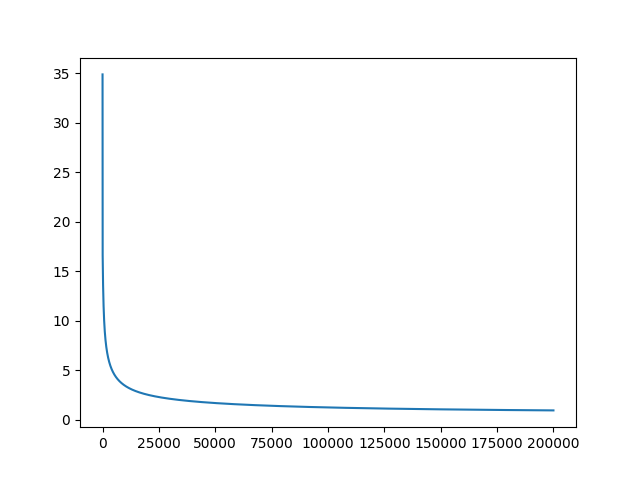
\includegraphics[scale=0.7]{HW2/logistic_regression_loss.png}
\end{center}

\noindent\textbf{Solution 3.3:}\\
\begin{center}
\begin{tabular}{ |c|c|c| } 
 \hline
 Gaussian generative model with... & Negative log-likelihood loss \\ 
 \hline\hline
 Shared covariance matrix & $-116.57191681902043$ \\
 \hline
 Separate covariance matrix & $-64.17309552244006$ \\ 
 \hline
\end{tabular}
\end{center}

The Gaussian generative model with separate covariance matrices has lower loss as the individual covariance matrices more accurately describe the variance observed in the training data in each class, allowing the classification to more closely fit the data. For example, the variance in Magnitudes of Dwarf stars is far greater than that of Giant stars or Dwarfs. Such detail is excluded when using a MLE for the shared covariance matrix, which takes a weighted average of the individual covariance matrices. Thus, using separate covariance matrices results in lower loss.

\noindent\textbf{Solution 3.4:}\\
\begin{center}
\begin{tabular}{ |c|c|c| } 
 \hline
 Model & Class of star with Mag. = 6 and Temp. = 2 \\ 
 \hline\hline
 Logistic Regression & Giant \\
 \hline
 Shared Covariance Gaussian & Giant \\ 
 \hline
 Separate Covariance Gaussian & Dwarf\\
 \hline
 KNN Model with k=1 & Dwarf\\
 \hline
 KNN Model with k=3 & Dwarf\\
 \hline
 KNN Model with k=5 & Dwarf\\
 \hline
\end{tabular}
\end{center}

There are two ways in which we can interpret the trustworthiness of the models:
\begin{enumerate}
    \item 4 of the models predicted the star with Magnitude = 6 and Temperature = 2 was a Dwarf star, while only 2 said it was a Giant star. Given the majority of models classified the star as a Dwarf, we can argue that these models are more trustworthy than the others which classified the star as a Giant.
    \item The decision boundaries in the logistic regression model and in the generative Gaussian model with shared covariances are quite similar, but are dissimilar to the separate covariances equivalent or kNN models. Since we have managed to create similar decision boundaries with two completely different models, both of which classify the star with Magnitude = 6 and Temperature = 2 as a Giant, we could arguably trust the models producing Giant predictions more.
\end{enumerate}
Therefore, we cannot definitely conclude which model is the most trustworthy using just these classifiers.

\newpage
%%%%%%%%%%%%%%%%%%%%%%%%%%%%%%%%%%%%%%%%%%%%%
% Name and Calibration
%%%%%%%%%%%%%%%%%%%%%%%%%%%%%%%%%%%%%%%%%%%%%
\subsection*{Name}
Ben Ray

\subsection*{Collaborators and Resources}
Whom did you work with, and did you use any resources beyond cs181-textbook and your notes?\\
Worked with Ty Geri, Elias Nuwara, and Angela Li\\
CS 181 Office hours

\subsection*{Calibration}
Approximately how long did this homework take you to complete (in hours)?\\
26


\end{document}
